\chapter{Estratégias do Jogo Oficial} 

Há quem diga que UNO é um jogo de pura sorte, e há pouco espaço para a intervenção estratégica no jogo; que há muitas variáveis e que, portanto, é inútil tentar agir conscientemente em relação ao jogo. Acredito que não, e que existem várias estratégias a serem empregadas.

Esta seção se divide em três: Em primeiro lugar, daremos uma olhada em estratégias gerais, que são importantes guias de ação. Quando se se joga em dupla, entretanto, algumas diferenças devem ser levadas em conta; olharemos estas estratégias em particular e, por fim, pensaremos em estratégias e na dinâmica do jogo de parceiros.

\section{Estratégia Geral}

A dinâmica do jogo em suas regras oficiais é simples: você deve descartar suas cartas o mais rápido possível, não apenas para ganhar o jogo, mas para evitar conceder ao eventual vitorioso um grande número de pontos.

Ao mesmo tempo, você tem a sua disposição cartas que prejudicam os outros adversários, e deve procurar usá-las também para impedir que eles vençam. Existem cartas que não só prejudicam os adversários, mas também te dão benefícios essenciais, como as cartas Curinga.

Jogar estas cartas ofensivas no começo do jogo não é a melhor estratégia possível, uma vez que as cartas de todos os jogadores ainda estão equilibradas, e isso pode acabar dando também poder ofensivo a eles. Além disso, perde-se a oportunidade de usá-las quando uma delas for essencial para impedir a vitória alheia ou alcançar a própria mais adiante na partida. Por outro lado, se as cartas forem conservadas por muito tempo na mão, uma melhor estratégia de um adversário pode prevalecer, e muitos pontos serão entregues a ele.

Neste cenário, torna-se óbvio que criar uma boa estratégia, num jogo individual, significa uma \textbf{escolha do tempo certo, em face da situação dos adversários, para jogar as cartas certas e proporcionar uma continuidade ao seu jogo}. Aspectos da formação dessa estratégia serão discutidos a seguir.

\subsection{Continuidade do Jogo}

Uma característica importante a notar é tentar o máximo possível provocar a \textit{continuidade} do próprio jogo. Isto significa jogar de um tal modo que a sua próxima vez seja vantajosa para sua estratégia geral.

Ao jogar uma carta, você deve fazê-lo esperando que, quando for sua vez de jogar novamente, você seja capaz de jogar outra carta (e até planejar qual carta será) ao invés de não ter mais opções e ser obrigado a comprar outra carta.

\subsection{Escolha das Cartas em Virtude da Continuidade}

Suponha um jogo em que você tenha as seguintes cartas à mão\footnote{Cartas escolhidas aleatoriamente, a partir de um baralho de UNO real.}:

\begin{figure}[!h]
\centering
\fbox{
\includegraphics[scale=0.5]{fig2.png}}
\caption{Pular Azul, Inverter Azul, Comprar Duas Cartas Verde, 6 Azul, 1 Amarelo, 6 Azul, 2 Azul}
\end{figure}

Supondo que todos os seus adversários tenham também 7 cartas, e que a carta na pilha de descarte seja um \textbf{2 Azul}. Que carta deveria ser jogada?

Você tem à sua disposição 5 cartas azuis. Duas delas são cartas de ação, que certamente serão muito mais úteis em rodadas vindouras, uma vez que ninguém está em real posição de vencer o jogo neste momento. Neste caso, sobram apenas três alternativas: dois 6 e um 2.

Pode parecer uma escolha irrelevante, mas imagine a próxima rodada. Se um 2 for jogado, mesmo não sendo azul (na verdade, é impossível que ele seja azul, afinal você sabe onde estão os dois 2 azuis do baralho e sabe que não existem outros), você terá um dois para jogar, e assim você não precisará comprar uma carta se for um 2 vermelho, por exemplo. Mas, se você jogar um dois agora, nesta rodada, não terá essa possibilidade mais adiante.

Contudo, se nesta rodada você jogar um 6 azul, na próxima rodada não só você terá um 2 azul para jogar caso um 2 vermelho seja posto no descarte, como também terá um 6 caso algum 6 seja jogado. Ao ter duas cartas iguais, você pode jogar uma delas e ainda assim conservar a outra, aumentando as chances de você poder dar continuidade ao seu jogo.

Quis o futuro\footnote{A carta escolhida foi aleatória, assim como a mão de exemplo, e a partir de agora não farei mais esta observação. Todas essas cartas foram escolhidas aleatoriamente.} que na sua próxima vez, a carta do descarte seja um 2 verde. Portanto, com efeito, o fato de você ter jogado um 6 azul, e não um 2 azul, faz com que você tenha opções: pode descartar um 2 azul ou um Comprar Duas Cartas Verde. O adversário à sua esquerda (neste sentido do jogo, vamos considerar que ele é o próximo a jogar depois de você) tem 6 cartas; talvez não seja a melhor hora para jogar esta carta. Se a sorte e as estratégias dos adversários vão favorecer esta espera, só o tempo dirá.

Você joga o dois azul. Na sua próxima rodada, a carta é um 6 amarelo. Aqui chegamos a uma decisão crucial, a decisão entre um número e uma cor.

Você poderia optar por jogar o 6 azul ou o 1 amarelo. Ao jogar o 1 amarelo, você deixa de ter qualquer carta número 1, e qualquer carta amarela. Ao jogar o 6 azul, deixa de ter qualquer 6 --- mas conserva suas cartas azuis.

Em qualquer mão, sem considerar outros atributos da situação, escolher a cor sobre o número é sempre o certo a fazer. Há muito mais chance de a próxima carta na sua vez ser alguma carta amarela do que um 6 (existem 25 cartas amarelas no jogo, sem contar os curingas; em contrapartida, existem oito cartas 6 no baralho), portanto conservar o 1 e jogar o 6 seria o mais lógico.

Entretanto, há sempre outras coisas a levar em consideração. Aqui, ao descartar um 6 amarelo, todas as suas cartas azuis serão cartas de ação. Não é um problema absoluto, mas tudo depende sempre da situação. Em outros jogos (não envolvendo este exemplo) jogar uma carta azul pode ser apropriado. Por exemplo, se o próximo jogador estiver com apenas uma ou mesmo duas cartas na mão, e você \textit{deduziu} (devido a observações das rodadas anteriores; mais sobre isso adiante) que ele não tem cartas azuis na mão, você deve jogar a carta azul para impedir que ele se aproxime ainda mais da vitória. Entretanto, em situações normais de simples escolha entre número e cor, onde você acaba eliminando uma cor ou um número da sua mão, \textbf{escolha eliminar um número}.

O 6 azul é jogado. A próxima carta é um 5 azul; você ou inverte o jogo ou pula o próximo jogador. Note que, em qualquer situação, o efeito acaba sendo evitar que a próxima pessoa jogue. Contudo, outras variáveis precisam ser observadas.

Se você acredita que o próximo jogador na sequência atual possua cartas perigosas pra você, você não deve inverter o jogo, porque você passaria a ser o próximo depois da jogada \textit{dele}.

Por outro lado, se o jogador que joga após o próximo possua uma ou mesmo duas cartas, pular o próximo pode não ser uma boa ideia; afinal de contas, isso vai fazer com que aquele jogador com poucas cartas jogue diretamente. Permitir que o próximo jogador faça uma interferência, mudando, talvez, a cor da carta no descarte, ou mesmo invertendo o jogo, fazendo com que ele compre mais cartas, etc, pode ser uma boa ideia. Pode não ser uma boa ideia se o próximo jogador \textit{também tenha poucas cartas}.

Se realmente não for desejável pular o jogo ou invertê-lo (ou se ainda você deseja conservar a carta especial para depois), lembre-se que você pode optar por não jogar uma carta que você possa jogar, e compre uma carta ao invés disso (só que, uma vez comprada uma carta, você não poderá jogar uma carta que já possuía antes, apenas a nova carta).

Vamos continuar, supondo que você tenha invertido o jogo. A próxima carta é um 1 verde. Considerando que a sua mão agora é formada por um Comprar Duas Cartas Verde, um 1 Amarelo e um Pular Azul, você tem novamente o dilema entre número e cor --- exceto que agora qualquer jogada sua vai eliminar uma cor da sua mão. Lembre-se, contudo, que provavelmente os seus adversários também agora possuem poucas cartas na mão. Seria uma boa ideia fazer o próximo jogador comprar duas cartas.

Neste ponto do jogo, é difícil criar estratégias com base na continuidade; imagine a situação corrente. Você possui apenas um Pular Azul e um 1 Amarelo. Uma carta não oferece continuidade à outra; o máximo a fazer é esperar que a dinâmica de jogo faça sua mágica e mude substancialmente a carta no descarte, a ponto de o seu amarelo virar um azul, ou a sua carta azul se transformar no amarelo. Entretanto, perceba: se você jogar o Pular Azul, menos pessoas jogarão na rodada, diminuindo a chance de que a cor na pilha do descarte mude.

Vimos que é importante jogar de um modo a maximizar as suas chances de continuar jogando, sem parar para comprar mais cartas. Vimos também que é importante descobrir a hora oportuna de descartar as cartas não-numéricas, sendo desvantajoso o uso precoce, porém perigoso o contínuo atraso do uso.

A chance de formar uma estratégia coerente baseada no princípio da continuidade diminui com o número de cartas. Portanto, quanto maior o número de cartas e, em especial, o de cartas de ação, maior o poder de gerenciar o jogo. Pode-se deduzir que uma estratégia vitoriosa passa por tentar \textit{gerenciar} o jogo no início, mas não se deixar levar pela ilusão de que controlar as coisas basta: quanto mais você tenta controlar o jogo, mais os adversários lutam para fugir a esse controle, e as estratégias de fuga são fundamentais para levar à vitória. Saber a hora de abandonar o gerenciamento para resistir ao gerenciamento alheio é, em resumo, a qualidade da estratégia geral do jogo.

\section{O Jogo dos Outros}

A continuidade, levando em conta apenas as próprias cartas e as probabilidades absolutas sobre que cartas podem determinar a sua próxima jogada, acaba contando pouco se não for complementada pelo conhecimento dos \textit{outros} jogadores: suas cartas e suas prováveis estratégias; a probabilidade relativa sobre que cartas determinarão sua própria vez no turno. É um conhecimento útil para escapar ao gerenciamento, e também para gerenciar o jogo, que é um princípio fundamental de toda boa estratégia.

Saber, diretamente, as cartas dos outros, é impossível\footnote{Existem exceções, como regras alternativas ou quando alguém desafia um jogador que acabou de jogar um Curinga Comprar Quatro Cartas na mesa.}. Entretanto, sempre existem modos criativos de roubar no jogo --- e modos inteligentes de descobrir, indiretamente, as possíveis cartas dos seus adversários. Esses métodos serão explorados a partir de agora.

\subsection{Segurança}

Não vou, neste guia, aconselhar a desonestidade. Além disso, explicá-la é trivial e tentar catalogar todos os métodos para ver as cartas dos adversários, impossível. O que se pode fazer é advertir os jogadores quanto a condições de jogo que favorecem a atitude desonesta:

\begin{description}
\item[Superfícies Espelhadas]{É preciso um cuidado especial quanto à escolha do lugar do jogo: espelhos e vidros podem proporcionar a certos jogadores posições privilegiadas em que podem ver as cartas de outros jogadores menos afortunados.}
\item[Interrupções Inocentes]{É natural que os jogadores sintam sede e fome, mas levantar no meio de uma partida para pegar água, quando para isto é necessário passar por detrás de vários jogadores, é suspeito: é possível instituir uma regra em que a partida é pausada para que o jogador possa fazer o que quer, ou, no mínimo, os jogadores devem ser espertos o suficiente para abaixar as cartas quando outros deles passarem por lugares específicos.}
\item[Postura e Relaxamento]{Uma coisa, contudo, é muito comum, especialmente em jogadores novatos e casuais: uma má postura dos braços ou do próprio corpo combinada com uma má disposição de lugares para os jogadores pode fazer com que, mesmo acidentalmente, outros jogadores vejam suas cartas. É preciso ter consciência disso e cuidado com o ângulo de visão dos adversários. Em geral, é possível prevenir isso se acostumando a deixar as cartas sempre na mesa, viradas para baixo, enquanto não for sua vez de jogar. Isso, contudo, pode ser problemático quando usado em conjunto com certas regras alternativas apresentadas mais adiante. Tome cuidado, também, com superfícies espelhadas e mesas transparentes, como foi dito anteriormente.}
\end{description}

Além disso, é importante também lembrar uma técnica de ``roubo'' no jogo muito utilizada. Ao descartar uma carta, o jogador descarta na verdade duas, escondendo uma embaixo da outra, como se apenas uma carta tivesse sido de fato posta na pilha de descarte\footnote{Outro perigo, real apenas se a Regra do Descarte Rápido ou das Duplicatas for aplicada (ver adiante, nas páginas \pageref{descarterapido} e \pageref{duplicatas}, respectivamente), é de o jogador jogar duas ou mais cartas ao mesmo tempo, de forma irregular.}. 

\subsection{A Mente dos Outros}

Ao ``ler'' os jogadores e os ``sinais'' que eles mandam, é possível saber não que cartas exatamente possuem, mas determinar uma probabilidade de que sejam cartas boas ou ruins, ou de que a carta no monte de descarte lhes agrade ou não.

Em geral, você não precisa ser um \emph{jogador experiente} para entender tais sinais: você precisa captar bem as pessoas e sua linguagem corporal. Isso pode ser aprendido, mas algumas pessoas têm esse talento de decifrar emoções e intenções observando as feições e atitudes das pessoas. O objetivo desse guia não é ensinar linguagem corporal a jogadores de UNO; existem outras obras disponíveis para aprender isso. Contudo, há algumas constantes e correlações a que devemos estar atentos:

Em geral, você deve primeiro determinar o tipo de jogador com o qual você está lidando. Algumas dessas perguntas podem ajudá-lo a desvendar aspectos essenciais da psicologia dos adversários:

\begin{itemize}
\item{Ele parece competitivo? Perder seria fonte de irritação e raiva? Ou isso lhe seria, em última instância, irrelevante?}
\item{Ele parece habilidoso? Tem noção de estratégias de jogo, de tudo aquilo que ele pode fazer com as cartas que têm à mão? Ou joga de um modo quase arbitrário, aleatório?}
\item{Quando fica quieto e não propenso a risadas, falatórios e brincadeiras, seu jogo está ruim e sua estratégia, precária? Ou é apenas seu estado natural, seu estilo de jogo?}
\item{Por fim, tudo isso é o que ele aparenta ser ou o que ele é? Ele é capaz de dissimular emoções ou você pode extrair de seus sinais físicos imprudentes a verdade sobre sua situação no jogo?}
\end{itemize}

Uma vez que você conhece seus oponentes (o que é mais fácil quando você joga com pessoas que conhece bem, como amigos e familiares) você pode tentar decifrá-los --- se sua estratégia foi reforçada ou precisa agora ser reestruturada; se seu jogo é favorável e propício ou desarticulado --- em alguns momentos-chave:

\begin{itemize}
\item{Ao comprar uma carta: como reagem?}
\item{Quando a cor da carta que eles jogaram na sua última vez muda durante a rodada: como eles lidam com a transformação? O que estavam esperando que acontecesse?}
\item{Uma mudança sutil, muito relativa e complexa: como eles reagem às reações à carta que jogaram na última rodada? Um jogador está tentando, em suma, \textbf{gerenciar} o jogo ou \textbf{escapar} ao gerenciamento? Por exemplo, ao jogar uma carta amarela, ele o fez por querer que um outro jogador comprasse uma carta ou por outras razões, que dizem mais respeito às cartas que ele mesmo possui?}
\end{itemize}

Esse tipo de observação pode levá-lo a descobrir quais jogadores possuem boas cartas no momento --- ao gerenciar o jogo, você deve procurar atacá-los, impedindo que vençam. Ao entender quais jogadores estão procurando controlar o jogo, você pode querer evitá-los, ou mesmo enganá-los, fazendo-os acreditar que você não está bem no jogo --- ou fazendo-os acreditar nisso com atitudes como comprar uma carta, mesmo podendo jogar alguma da sua mão.

\subsection{As Cartas dos Outros}

\label{leituradosjogadorescartas}

Agora, deixando de lado os aspectos psicológicos dos jogadores e pensando na leitura objetiva das \textit{cartas} que os adversários têm, chegamos a um pequeno conjunto de procedimentos e observações que podem nos ser úteis.

\subsubsection{A Compra}

Em primeiro lugar, é sempre importante memorizar o momento em que os jogadores \textit{compram} cartas. Uma compra dissimulada é sempre arriscada, então aprenda a tomar as compras como ótimos indicadores das cartas do adversário. Se um adversário compra uma carta quanto, por exemplo, um 8 vermelho está na pilha de descarte, isso significa que, naquele momento, ele não possui oito algum, tampouco alguma carta vermelha. Também é relativamente seguro supor que a carta comprada não tenha sido 8, nem vermelha, caso contrário ela teria sido jogada pelo adversário.

Isso é importante porque, à medida que o jogo prossegue, pode ser você o jogador a usar um curinga, e o adversário em questão pode ter uma ou duas cartas na mão. Se você souber que ele não possui nenhuma carta vermelha na mão, pode definir o curinga como vermelho e ele então não poderá jogar (a não ser que conserve um curinga na mão).

Esse tipo de memorização é crucial. Entretanto, quanto menos preocupados formos em ganhar, menos nos preocuparemos com detalhes: muitas vezes é difícil lembrar da cor que o adversário não tem, e é ainda mais raro lembrar dos números. Mas se você treinar e estiver interessado, poderá desenvolver uma melhor técnica para se lembrar desse tipo de detalhe.

\subsubsection{O Uso do Curinga}

Outro momento importante que pode passar despercebido é o momento em que um Curinga Comprar Quatro Cartas ou um simples Curinga é jogado: eles (quase) equivalem a uma compra, no sentido de que evidenciam que \textbf{cor} de carta o adversário \emph{não} possui --- a não ser que ele esteja blefando, é claro. Além disso, é preciso prestar atenção também à cor de carta que o jogador pede ao jogar um Curinga: isso é geralmente algo que possui valor para ele e suas cartas atuais.

\subsubsection{A Espera}

Se o adversário demora a jogar e tem poucas cartas na mão, é muito provável que ele não esteja apenas com dificuldades para fazer sentido das cartas que tem à mão: ele está \emph{tomando uma decisão}. Em geral a decisão costuma ser entre:

\begin{itemize}
\item{Jogar a única carta na mão que pode ser jogada ou um Curinga; ou}
\item{Jogar uma carta que elimine a cor na mão ou elimine o número.}
\end{itemize}

Este último caso merece uma melhor observação: o que ele exatamente significa? Supondo que a carta na pilha de descarte seja um Cinco Vermelho. O jogador tem apenas duas cartas na mão: um Cinco Verde e um Oito Vermelho.

Ou seja, mesmo que você não saiba exatamente quais cartas estão na mão dele, a partir da indecisão você já pode supor que sejam um Cinco e uma carta vermelha\footnote{Ou uma destas cartas é um Curinga, e é esta a fonte da indecisão, como esclarecido acima.}. Se ele jogar um cinco, você já sabe que a carta que ele têm em mãos é vermelha. Se ele jogar o Oito Vermelho, você já sabe que a carta nas mãos dele é um Cinco. De qualquer forma, é uma informação valiosa.

Esse conjunto de técnicas será, é claro, usado contra você no jogo. Existem formas de subvertê-los, usando as suposições e memorizações dos adversários contra eles. Você pode jogar comprar uma carta sem necessidade, blefar no uso de um Curinga, pedir uma cor que você não tenha depois de jogar um Curinga e esperar para jogar mesmo sem que uma decisão precise ser feita. A maioria dessas formas de manipulação será discutida mais abaixo na seção de estratégias específicas (ver página \pageref{estesp}), e pode vir a ser alterada com o uso de regras alternativas (ver, por exemplo, a Regra do Desafio Polivalente, na página \pageref{desafiopolivalente}).

\subsection{Memorização das Cartas}

\label{memorizacaodascartas}

A informação sobre a cor de carta --- e os números ou símbolos --- que um adversário não possui é importantíssima, mas ela pode ser muito mais funcional se combinada com uma memorização completa de todas as cartas do jogo, analisando, assim, todas as possíveis mãos dos adversários e, à medida que o jogo progride, tentando descobrir especificamente quais cartas eles têm e não têm.

Como pode ser lido nas regras oficiais do jogo, o baralho de UNO possui 108 cartas. Memorize o número de cartas de cada tipo, e a cada carta decartada (e as que você sabe que estão na sua mão, ou as que você sabe que seu oponente não tem) você pode formar estatísticas: o que é mais \textit{provável} que seu adversário não tenha? Várias cartas vermelhas foram jogadas no descarte, mas poucas verdes. É mais provável que ele não tenha uma vermelha. E lembre-se de um detalhe que muitas pessoas não notam, mas pode fazer a diferença: todas as cartas numéricas possuem duplicatas (existem duas cartas 3 Verde, por exemplo) --- exceto as cartas de número \textit{0}. Outro dado interessante de lembrar é quantas cartas Comprar Duas Cartas ou quantos Curinga Comprar Quatro Cartas foram jogados.

Vimos, portanto, que é essencial balancear a continuidade e o tempo de gerenciamento de jogo (quando você gerencia e quando não gerencia. Também é importante não só pensar nas próprias cartas, mas nas dos adversários, prevenir contra desonestidades no jogo e ``ler'' os adversários. É também proveitoso lembrar de certas cartas jogadas para poder fazer cálculos sobre o jogo.

\section{O Estímulo Passional}

UNO é um jogo em que, quando jogado com leveza e por diversão, as emoções costumam vir à tona com a surpresa das reviravoltas inesperadas, a irritação do esquecimento da fugaz palavra ``UNO'' ou a frustração da falta de sorte com as cartas compradas.

Os jogadores tendem a muitas vezes agir passionalmente, a levar o jogo para o lado pessoal e a ter atitudes irracionais. Vamos procurar entender esta dinâmica, e como pode ser identificada, estimulada, e até certo ponto \textit{controlada}.

Como foi dito anteriormente, existem dois motivos para a ação consciente no jogo do UNO: o impulso de gerenciar o jogo e o impulso de escapar ao gerenciamento alheio; o foco no poder, no controle, ou na velocidade e na sagacidade para se esgueirar pelas frestras das estratégias alheias e, com sorte, dar o golpe final nos adversários.

Esses são impulsos \textit{conscientes}, atitudes de quem sabe o que está fazendo e como deve proceder para aumentar suas chances de vitória. Lado a lado com estas atitudes conscientes (exercidas em diversos níveis de proficiência) caminham no jogador impulsos inconscientes, \textit{posturas de jogo} que podem, durante momentos de falta de lucidez tática, transbordar e se transformar em \textit{modo de jogar}, \textit{escolhas sobre o jogo}.

Existem, em geral, dois impulsos inconscientes: a agressividade e a tranquilidade. Há vários tipos de alvos contra o qual eles surgem: uma outra dupla (quando o jogo é jogado em parcerias), um jogador em especial ou o próprio azar (alvo que não deve ser ignorado).

Pode-se dizer que a agressividade, a vontade de atacar e reagir ao que o cérebro quase instantaneamente rotula como uma ``óbvia conspiração feita de ódio e ressentimento'' (Não pode ser! Comprar mais quatro, \textit{de novo}?) seria o lado sem foco, sem concentração e inteligência, do instinto de gerenciar o jogo, controlar a dinâmica da partida. Por outro lado, a tranquilidade, a sensação de que o jogo é conduzido de maneira equilibrada, seria a contrapartida instintiva e sem foco da tentativa de não controlar o jogo dos outros, mas o seu próprio, tentando fazer sua própria estratégia vitoriosa ao escapar da linha de fogo cruzado dos inimigos.

O foco, a atenção, a \textit{racionalidade} das escolhas separa os impulsos instintivos dos impulsos racionais. Os quatro impulsos podem levar à vitória de algum modo, afinal vencer, neste jogo, não passa somente por criar uma boa estratégia, mas esse é o único fator que se \textit{sabe} que ajuda e a medida dessa influência é visível e controlável. Conhecer os impulsos irracionais faz parte da tentativa de incorporá-los à sua estratégia de jogo, seja ela no momento de um impulso de gerenciamento ou não.

Ao passo que a tranquilidade é um impulso insípido no que concerne à nossa estratégia, é a agressividade que é útil --- entender seus efeitos sobre os jogadores é importante, pois um jogador sob o efeito da pura tranquilidade (que é levemente diferente do impulso racional correspondente) vai adotar uma estratégia que o conduz, calmo como um Buda feliz, ao que lhe parece ser uma vitória --- ele apenas acompanha o fluxo que, caso não fosse interrompido pelas loucuras do jogo que todos bem conhecemos, levaria qualquer um, evidentemente, à vitória. De descarte em descarte, um dia se chega a ter nada na mão.

Já o jogador agressivo está sedento de sangue: ele pode até mesmo preferir sacrificar alguma oportunidade de melhorar seu jogo por qualquer chance que tenha de atacar seu agressor. Em outros casos, a raiva simplesmente o cega, impede que ele siga caminhos mais benéficos, que elevariam suas chances de vencer.

A agressividade tem origem em alguns pontos-chave do jogo:

\begin{description}
\item[Ficar muitas rodadas sem jogar]{Quando está prestes a jogar, o jogador anterior joga uma carta Pular, ou Inverter, e isso se repete fazendo com que ele fique muito tempo sem jogar. Em UNO, duas rodadas acabam significando uma terrível desvantagem.}
\item[Ser obrigado a comprar cartas por não ter o que jogar]{Ter que comprar cartas por não ter na mão nenhuma carta passível de ser jogada. Note que isso é diferente de \textit{escolher} comprar cartas; a raiva surge da falta de escolha. A raiva é tanto maior quando a compra é infrutífera, e o número de cartas na mão aumenta.}
\item[Ser obrigado a comprar muitas cartas por causa de punições]{Esquecer de dizer ``UNO'' ou outro motivo que cause punições.}
\item[Ser obrigado a comprar cartas por obrigação]{Cartas de compra (Comprar Duas, Curinga Comprar Quatro) são verdadeiras causadoras de úlceras quando são jogadas repetidamente. A ideia de comprar 6 ou 8 cartas em duas ou três rodadas é um pesadelo para o jogador que não encara isso como uma oportunidade de gerenciar o jogo. Entretanto, quando há realmente pouca oportunidade de gerenciar o jogo, a raiva é mesmo muito difícil de controlar.}
\end{description}

Em alguns desses casos estímulos são necessários para que a situação desvantajosa gere uma raiva que possa obscurecer a mente do adversário ou fazer com que ele resolva atacar diretamente uma outra pessoa. Esse estímulo pode ser uma risada quando o incauto azarado comenta que vai mal, ou, mais fundamentalmente --- quando isso é possível --- comentários que indiquem a \textit{culpa} de alguém. Por exemplo, quando uma pessoa compra várias cartas em virtude de cartas Comprar Duas, é possível tripudiar da má fortuna do jogador e sugerir que o atacante que jogou essas cartas o fez de \textit{propósito}, por \textit{maldade}. Às vezes isso é verdade, mas às vezes o jogador até preferiria guardar as cartas, mas isso não seria possível sem ter que \textit{comprar} cartas, o que seria mais desvantajoso.

Os alvos, e os efeitos que causam, são:

\begin{description}
\item[Outro jogador ou outros jogadores]{O adversário em situação de infortúnio vai simplesmente tentar se vingar da melhor maneira que tem à disposição. Se ele possuir uma carta de Inversão e uma Comprar Duas Cartas, vai tentar fazer de tudo pra inverter o jogo e poder agora fazer seu algoz comprar as cartas --- e isso por vezes inclui comprar cartas desnecessariamente e fazer escolhas de jogo que até mesmo quebrem a própria continuidade.}
\item[O próprio azar]{Ao ter raiva do próprio azar, muitas vezes o jogador desiste de formar uma estratégia e simplesmente ``joga qualquer coisa'', descrente de que possa vencer o jogo. Desanimar o jogador, incutir nele a ideia de que a partida está perdida --- ou de que alguém é culpado pela sua compra de cartas, o que faz com que voltemos ao primeiro ítem desta lista --- é uma forma de se livrar, sem muito esforço, de um adversário que, sem tal desânimo, poderia tentar atrapalhar os outros sempre que possível.}
\end{description}

Para evitar se tornar alvo de jogadores vingativos, procure fazer o seguinte:

\begin{description}
\item[Não concentre ataques]{Tente não atacar um mesmo jogador seguidamente; dê no mínimo um espaço de uma rodada entre uma carta desvantajosa para ele e outra.}
\item[Não chame atenção]{Não faça um ataque declarado a um adversário ou comente suas intenções de fazer com que alguém compre mais cartas ou se atrapalhe no jogo, ou alguém experiente sequer precisará incitar um jogador contra você.}
\item[Justifique-se]{Há um velho ditado que diz que você nunca deve se explicar: seus inimigos não acreditarão, e quem for seu amigo não exigirá explicações. No UNO, declarar inocência pode funcionar. Dizer que era a única escolha (ou mesmo o mais verossímil ``era a única escolha sensata'') pode amenizar a situação.}
\item[Não blefe]{Blefar tem um desdobramento lógico perceptível para todos os jogadores: se ele mentiu, é porque \textit{queria} que o oponente comprasse as cartas. Isso chama a atenção e causa agressividade. Blefar, uma hora ou outra, torna-se importante, mas se você não quiser um comportamento agressivo contra você, prefira blefar raramente ou não blefar.}
\end{description}

É importante lembrar duas coisas: mesmo nas situações mais informais, alguém que tenta sempre jogar uma pessoa contra outra logo será reconhecida por tal característica, e mais adiante tudo que disser nesse sentido será ignorado. Portanto, como quase toda tática não-discreta contida neste guia, o uso repetido leva à ineficiência.

Além disso, é crucial lembrar que a agressividade mencionada aqui é puramente lúdica; UNO é apenas um jogo e as rivalidades devem durar apenas enquanto o jogo durar, devendo ser encaradas como um aspecto natural e \textit{divertido} do jogo.

\section{Estratégias Específicas}

\label{estesp}

Existem certas estratégicas --- mais provavelmente \textit{táticas} --- que são empregadas durante um jogo oficial que vale a pena discutir e apresentar, ainda que não façam parte de um grande sistema de pensamento acerca da administração de uma partida de UNO.

\subsection{O Curinga Surpresa}

\label{curingasurpresa}

É muito comum querer guardar uma carta curinga para a última rodada. As vantagens são óbvias: se for possível chegar a um ponto em que você tenha apenas uma carta na mão, e essa seja um curinga, a única coisa que pode impedir você de ganhar o jogo é uma carta Comprar Dois (ou Curinga Comprar Quatro) do jogador anterior a você. Caso contrário, você pode vencer com qualquer carta na pilha de descarte.

Existem dois problemas com esta estratégia: em primeiro lugar, você vai precisar de um pouco de sorte para chegar a ter apenas o curinga na mão. Como mostramos anteriormente, o seu poder de dar continuidade ao próprio jogo pode ser enorme quando você tem várias cartas, mas diminui progressivamente à medida em que você vai usando o seu poder, \textit{i.e.} descartando as cartas. Quando você chega a ter duas ou três cartas na mão, você acaba dependendo muito das jogadas dos outros jogadores; é preciso que a carta na pilha de descarte na sua vez seja perfeita para que você possa guardar o curinga até o final. Isso nem sempre acontece, e, quando não acontece, você é obrigado a comprar uma carta se quiser continuar esperando pelo momento oportuno.

Isso geralmente acaba mal, e aí temos nosso segundo problema: alguém com uma estratégia diferente vence o jogo antes de você e acaba ganhando 50 pontos por causa do seu curinga não descartado. Temos então que é uma estratégia arriscada, mas plausível e, quando bem executada, muito eficiente.

\subsection{``Olha o Avião'' Longo}

\label{aviaolongo}

O cenário: você está com duas cartas na mão. Uma delas é o curinga; com o jogo do jeito que está, você precisa descartá-lo para seguir em frente, ou precisará comprar outra carta --- e outros jogadores já estão tão avançados quanto você no jogo. Você resolve não tentar ``O Curinga Surpresa'' (ver acima, página \pageref{curingasurpresa}), e joga o curinga. Você possui, digamos, um 3 amarelo na mão. E agora você decide a cor.

\begin{wrapfigure}{o}{0.25\textwidth}
  \begin{center}
    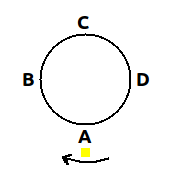
\includegraphics[scale=0.5]{fig3.png}
  \end{center}
  \caption{Quando o jogador fica com apenas uma carta na mão, até ele voltar a jogar a cor pode ter se modificado. Ao pedir outra cor, ele pode confundir os adversários.}
\end{wrapfigure}

Temos, antes de tudo, de ver um dilema anterior a essa tática: você deve evitar que os adversários ganhem; gerenciar o jogo. Dessa forma, se algum adversário já estiver com apenas uma carta na mão você deve exigir na sua carta curinga uma cor que você saiba que ele não tenha (ver ``As Cartas dos Outros'' acima, na página \pageref{leituradosjogadorescartas}).

Entretanto, se este não for o caso, você deve exigir a cor amarelo, na lógica da continuidade do jogo. Entretanto, dependendo do número de jogadores, esperar que na sua próxima vez a cor na pilha de descarte continue sendo amarela é, em geral, uma atitude que leva à frustração. Uma tática que parece uma aposta cega é exigir uma outra cor, não a que você tem na mão: exija azul, por exemplo. Como a tática costuma funcionar? Um jogador percebe que você pediu a cor azul, e que você, portanto, \textit{deve ter} uma carta azul na mão. Ele mudará a cor --- para, há uma grande chance, amarelo --- para impedir que você vença, e você enfim revela que enganou a todos ao jogar uma carta amarela na sua vez e ganhar o jogo.

Uma consequência curiosa do uso repetido e insistente dessa estratégia é que seus oponentes podem perder a fé na coerência das suas escolhas, e eventualmente prestarão menos atenção às suas atitudes, deixando de tentar ``ler'' a sua atitude e suas cartas --- porque julgarão isto uma tentativa inútil, já que você vai sempre pedir o que não tem. Contudo, essa estratégia, como mencionado, é arriscada: é mais provável que você perca mais do que ganhe ao usá-la repetidamente.

Essa é a variante ``Longa'' do ``Olha o Avião''. Existe uma variante que pode ser empregada em um jogo em parceiros, a ``Curta'', que veremos mais adiante (página \pageref{aviaocurto}).

\subsection{Jogue o Zero, Mantenha o Zero}

O zero é uma carta especial no jogo: existem menos zeros do que outros números no baralho. No final da partida, o zero não conta pontos para o adversário. A partir da primeira constatação, vemos que, teoricamente, descartar o zero é uma boa estratégia durante a partida: você vai ter uma melhor continuidade se conservar na mão cartas que te darão maior possibilidade de continuar jogando. Contudo, se um adversário ganhar, uma de suas cartas não vai lhe dar nenhum ponto.

O que fazer? Bem, é uma questão de momento. Se você tem mais esperanças de vencer o jogo, está numa situação favorável, não arrisque e livre-se do zero. Caso a vantagem seja do oponente, conserve-o.

\subsection{O Consumismo}

\label{consumismo}

Comprar cartas é algo que, em teoria, deve ser evitado a todo custo. Afinal, o objetivo do jogo é se livrar das cartas à mão; você compra cartas quando não há carta que você consiga jogar no momento (o que parece uma irônica punição da justiça ``uno-versal'' a uma possível estratégia ruim) ou --- o que deixa óbvio quão ruim isso é --- quando é punido por algo como não dizer ``uno'' ou jogar errado, etc.

Entretanto, há momentos em que comprar uma carta pode ser uma boa estratégia: nos momentos em que você assume o gerenciamento do jogo, ou seja, pretende controlar, interferir nos outros jogadores.

Se a vez é sua e o próximo jogador tem apenas uma carta na mão --- e você não tem nenhuma carta que possa impedi-lo de jogar --- por que não arriscar e comprar uma carta? Você se distancia um pouco mais da vitória, mas caso você compre algo útil, também se afasta da derrota iminente\footnote{Os riscos de se fazer isso, tentando prever as chances de conseguir uma carta útil, podem ser calculados grosseiramente (ou de forma precisa, dependendo da pessoa), como já visto na seção ``Memorização das Cartas'' acima, página \pageref{memorizacaodascartas}.}.

Comprar cartas pode ser útil para se munir de cartas de ação, que ajudam a gerenciar o jogo, ou mesmo de cartas que melhorem a sua disponibilidade de cores à mão. Você pode fazer isso enquanto a partida ainda está ``fria'' --- quando uma carta a mais não é assim tão relevante.

Outro motivo para comprar cartas pode ser também a vontade de reservar uma carta para mais depois --- mais ou menos como ocorre com a estratégia do ``Curinga Surpresa'' mencionada acima na página \pageref{curingasurpresa} --- mas, em contrapartida, não tem nada para jogar a não ser a carta que deseja guardar. A regra do jogo diz que uma compra é necessária; no mínimo você pode jogar a carta que comprou caso ela seja compatível com a carta da pilha de descarte no momento.

Assim, existem vários motivos para comprar cartas espontaneamente, não apenas por necessidade. Esteja alerta para estes motivos, que podem dizer muito sobre o jogo dos seus adversários --- não é porque eles compram uma carta que eles ``não têm a cor pra jogar''.

\subsection{Trébuchet Longo}

\label{trebuchetlongo}

Em um jogo de muitas pessoas, o Trébuchet (como encontrado na internet) é o uso de uma situação desvantajosa em geral\footnote{Na verdade, alguns jogadores fazem uma distinção entre o Trébuchet, que é a situação de azar em que todos os jogadores não tem o que jogar e são obrigados a comprar, e um falso Trébuchet, em que um jogador pode jogar, mas não quer fazê-lo. Esse último caso é estrategicamente valioso, portanto é deste de que vamos tratar agora.}, mas não exatamente para si mesmo, para gerenciar o jogo.

\begin{wrapfigure}{i}{0.35\textwidth}
  \begin{center}
    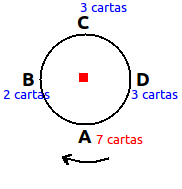
\includegraphics[scale=0.6]{fig4.png}
  \end{center}
  \caption{Você tem uma carta que pode ser jogada. Se você \emph{não} a jogar, possivelmente todos os jogadores comprarão uma carta. Por que jogá-la, então?}
\end{wrapfigure}

Ocorre que, em um número surpreendentemente considerável de partidas (sendo mais frequente com menos jogadores, como apenas 3 ou 4), vai haver um momento em que a última carta de uma cor e de um número ou tipo serão jogados; nenhum jogador vai ter em mãos alguma carta que possa ser jogada. Dessa forma, todos os jogadores comprarão cartas durante uma, duas, três ou até mesmo quatro rodadas até que finalmente alguém consiga comprar uma carta útil e possa jogá-la.

Acontece que essa situação, tecnicamente desvantajosa para todos, acaba sendo mais desvantajosa para alguns do que para outros; pessoas que têm alguma estratégia, alguma esperança de continuidade (ainda aliada, talvez, à estratégia ``Olha o Avião'' acima) acabam se prejudicando mais do que outras que não teriam nenhuma jogada que não fosse guiada pela sorte caso o jogo continuasse. Se você é uma dessas pessoas, essa estratégia --- ou falta de uma --- é ideal.

Suponhamos que uma rodada já tenha se passado desde que aquele 4 vermelho foi jogado na pilha de descarte; ninguém consegue tirar ele dali. É uma partida de quatro jogadores, você vai comprar a segunda carta, iniciando a segunda rodada de compras --- e, coincidentemente, você compra um quatro azul. Mas os outros jogadores, você percebe, estão em melhor situação que você. Admita, você não tem uma boa estratégia formada. Então, por que ajudar os outros jogadores? Por que dar a eles a chance de continuar, retomar suas estratégias? Ignore que você comprou uma carta que possa ser jogada. Continue comprando --- é claro, contanto que os outros também comprem. Duas ou três rodadas depois todos vão estar em pé de igualdade novamente, e você pode refazer sua estratégia, com cartas que abram o seu leque de possibilidades.

Esta é a variante longa do Trébuchet; existe uma variação ``Curta'' (para jogos apenas com dois jogadores, vista na página \pageref{trebuchetcurto}) e uma variante ``Dupla'' (para jogos com parceiros, vista na página \pageref{trebuchetduplo}), que serão abordadas mais adiante.

\subsection{Pontos Extras}

Uma estratégia interessante consiste em deixar para a última carta a ser descartada um Comprar Dois (ou um Curinga Comprar Quatro, o que de certa forma caracteriza um Curinga Surpresa, mas esta estratégia é um pouco diferente), pois, de acordo com as regras oficiais, se uma vitória for alcançada através de uma carta que force o próximo jogador a comprar, o próximo jogador em questão \emph{deve} comprar as cartas para que elas possam ser contadas no final da partida.

\section{Jogo em Dupla}

Como visto anteriormente nas regras oficiais (na página \pageref{oficiais}), o jogo em dupla conta com regras levemente diferentes. Afinal, as cartas ``Pular'' e ``Inverter'' não fariam sentido num jogo de duas pessoas. Nesse caso, essas cartas recebem a nova função de fazer com que o jogador que as joguem apenas jogue novamente.

A estratégia do jogo torna-se um pouco diferente: o foco na continuidade agora é ainda maior, levando em conta que não é tão provável que a cor da carta mude entre duas jogadas suas (em que apenas uma pessoa joga). Por outro lado, o fato de que as cartas especiais provocam a repetição do seu turno nos deixam com três tipos básicos de estratégia: uma assertiva, uma oportuna e uma flexível, e as três (especialmente as duas primeiras), apesar de mutuamente exclusivas, podem ser combinadas ao longo de uma partida (enquanto reação a uma estratégia bem sucedida do adversário). Além disso, ainda possuímos uma equivalente à ``Trébuchet'' analisada na seção anterior (página \pageref{trebuchetlongo}).

\subsection{Assertividade e Oportunismo}

Considerando que as cartas Pular, Inverter, Comprar Duas Cartas e Curinga Comprar Quatro Cartas fazem com que você jogue novamente, você deve ter em mente que qualquer quantidade desse tipo de cartas na sua mão faz toda a diferença do mundo, especialmente se elas puderem ser combinadas (i.e tiverem a mesma cor ou forem do mesmo tipo). Assim, ter três cartas Pular de cores diferentes é certamente melhor do que ter uma carta Pular, uma carta Inverter e uma carta Comprar Duas Cartas, as três de cores diferentes --- isso porque, quando aquela primeira série de cartas é jogada, é jogada em conjunto, uma atrás da outra, e faz com que você fique três rodadas à frente do jogador.

Contudo, a questão é: como e quando fazer uso dessas cartas que te deixam à frente? Já no começo da partida, para ganhar vantagem o mais cedo possível e liquidar o jogo? Mais perto do fim, arquitetando assim um ataque fulminante para qual o adversário não está preparado? Ou nenhum dos dois?

A primeira opção é a da Assertividade. Pode parecer óbvia a vantagem de começar o jogo já em vantagem; afinal, você sai na frente antes que os percalços do jogo façam com que você acabe comprando cartas e fique uma ou duas rodadas atrás do adversário --- o que pode ser fatal caso ele esteja se preparando para atacar de forma oportuna, o que veremos adiante.

O ataque assertivo possui uma função de desarmar o jogador adversário; se ele possui alguma combinação de cartas que possa dar esse tipo de vantagem a ele, ele vai ter que usar já para recuperar as rodadas que você já tomou dele; dessa forma, ele não pode mais guardar nenhuma carta na manga.

Guardar cartas na manga é o espírito do ataque oportuno. Construir as jogadas, basear-se na continuidade, até que a situação seja propícia e você despeje em sequência todas as cartas que façam você jogar novamente, ganhando, assim, o jogo, mesmo tendo três ou mais cartas na mão, por exemplo.

É claro que tanto a estratégia assertiva quanto a oportuna têm seus pontos fracos. Se a estratégia assertiva força o oponente a ``sair da toca'', você pode não gostar do que vai sair de lá; ele pode ter cartas muito mais vantajosas, e virar o jogo de um jeito espantoso, fazendo com que você fique numa situação muito pior do que se tivesse esperado, talvez, para realizar um ataque oportuno (embora se as cartas do adversário forem realmente boas talvez não se pudesse fazer muito quanto a isso).

Por outro lado, a estratégia oportuna funciona muito bem com um adversário passivo e que não tem um jogo bom. Você precisa de uma ótima continuidade de jogo para prosseguir constantemente rumo à utilização das cartas de ação que possam levá-lo à vitória. Um ataque oportuno do seu adversário, dado antes do seu, fará você perder. Um ataque assertivo vai forçar você a abandonar o ataque oportuno --- ou não, embora isso seja aconselhável.

Tanto o ataque assertivo quanto o oportuno se referem às cartas de ação jogadas como um contínuo; mas nem sempre essa jogada é a melhor saída (ou mesmo uma saída possível). Nesse caso, precisamos falar de uma terceira estratégia.

\subsection{Flexibilidade}

Por vezes, as suas cartas de ação não podem ser jogadas uma em cima da outra (proporcionando, assim, várias rodadas de vantagem de uma vez só), ou não é vantajoso fazer isso. Nesse caso, adotamos uma estratégia flexível.

Por vezes esta estratégia não é bem uma tática, e sim a falta de uma; uma pessoa com pouca habilidade não percebe direito as consequências de ataques assertivos e oportunos, e apenas joga as cartas de ação quando julga necessário --- mas não necessariamente em conjunto, e sim de uma em uma, usando-as com moderação. Inadvertidamente ou de propósito, esse pode acabar sendo, justamente por seu equilíbrio e sua prudência, o melhor tipo de estratégia.

É preciso reconhecer o momento certo de atacar para obter pequenas vantagens por dois motivos distintos: Ou o adversário já está em vantagem, e é preciso dirimi-la ou diminui-la; ou ele não está em vantagem, mas obter uma vantagem grande (de duas ou três rodadas) fará com que ele fique desesperado (como comentado acima) e ataque você também. Dessa forma, conquistar pequenas vantagens, carta a carta, é uma estratégia que evita o susto e o jogo baseado no medo; você não pode deixá-lo pensar que as coisas estão ficando ruins demais e, portanto, escapando a seu controle (incentivando-o, assim, quem sabe, a continuar com sua estratégia de ataque oportuno quando deveria imediatamente abandoná-la).

Lembrando que o jogo baseado na flexibilidade também oferece maiores oportunidades de continuidade (o que é um aspecto muito positivo) e, por vezes, é o único possível (quando não há muitas cartas de ataque, por exemplo).

\section{Estratégias Específicas do Jogo em Dupla}

Em um jogo entre duas pessoas, podemos dizer que existe uma estratégia específica a ser debatida:

\subsection{Trébuchet Curto}

\label{trebuchetcurto}

Assim como no jogo de 3 ou 4 pessoas, você pode chegar a uma situação muito desvantajosa para ambos os jogadores ao jogar em dupla. O Trébuchet é a estratégia em que você, mesmo podendo jogar uma carta e fazer o jogo continuar, prefere continuar comprando (contanto que o seu adversário também esteja comprando) para refazer o jogo.

Isso, é claro, não faz nenhum sentido a não ser que você esteja em situação de desvantagem. A compra de cartas durante duas, três ou quatro rodadas pode fazer uma diferença gigantesca --- tanto para o seu bem quanto para o seu mal.

Esta é a variante ``Curta'' do Trébuchet. Para a variante Longa (jogos com vários jogadores, vista na página \pageref{trebuchetlongo}), veja ``Trébuchet Longo'', acima. Para a variante ``Dupla'' (jogos com parceiros, vista na página \pageref{trebuchetduplo}), veja mais adiante.

\section{Jogo em Parceiros}

\label{jogoemparceiros}

As regras oficiais do UNO são particularmente displicentes quanto ao jogo em parceiros: ela apenas explicita que os parceiros devem sentar-se um à frente do outro. Mas o que é permitido que façam?

Essa ambiguidade não foi referida na seção que seria teoricamente apropriada pois não é uma ambiguidade entre duas coisas: a questão é muito aberta para ser posta em termos de fazer alguma coisa ou outra coisa. A questão é que não se sabe como funciona um jogo em parceiros; eles podem mostrar suas cartas uns aos outros, ou só podem fazê-lo clandestinamente, correndo o risco de fazer com que os adversários vejam as cartas? Podem fazer sinais e pedir por cartas e cores abertamente, ou isso é considerado um ``palpite'' (acarretando, assim, penalidades)?

Como um jogo em parceria não faria sentido se as equipes fossem descoordenadas, vamos considerar que a comunicação entre elas é aberta. Elas podem, portanto, inventar símbolos e formas secretas de comunicação para melhor coordenar suas ações --- afinal, de que adianta jogar em equipes se isso não acaba constituindo uma união tática de forças, mas sim apenas uma contagem conjunta de pontos?

Contudo, ver as cartas --- assim, de forma fácil, o tempo todo --- pode ser um pouco exagerado. Formar uma estratégia, gerenciar o jogo, pode ser, se assim for feito, fácil demais; além disso, a dinâmica do jogo pode ser um pouco prejudicada se o tempo inteiro os jogadores ficarem olhando as mãos uns dos outros para pensar em um jeito de atacar os adversários --- de forma implícita, o tempo (e o fato de que você deve jogar rápido para deixar o jogo interessante) faz parte da dificuldade em formar e executar uma estratégia.

Então, partindo do princípio de que esse é um manual de customização, crie suas próprias regras; eu, particularmente, recomendo que não sejam aplicadas penalidades para a comunicação entre membros da equipe, mas essa comunicação não deve ser constante e absoluta.

\subsection{Dupla Continuidade}

Se antes o importante era jogar de modo que a sua próxima vez seja vantajosa para sua estratégia geral, agora você tem uma outra variável: para que a sua parceria seja vitoriosa (contra uma outra), vocês precisam de uma única estratégia, utilizando-se do poder das duas ``mãos'' e jogadas --- duas pessoas em sintonia. A continuidade passa a ter outro sentido: o sentido de ser posta em ação em prol da estratégia geral, não apenas da própria.

Considerando, pois, um jogo de duas duplas, em que os jogadores A e C jogam contra os jogadores B e D\footnote{vamos considerar essas duplas com letras de ordem alternada, uma vez que as duplas não podem ficar em posições consecutivas na mesa.}, vamos imaginar um jogo-exemplo para darmos uma melhor ideia dessa questão da dupla continuidade (a continuidade que serve não apenas a si mesmo, mas à dupla).

\subsection{Escolha das Cartas em Virtude da Dupla Continuidade}

Pensar em escolhas de cartas que favoreceram a uma estratégia geral parece complexo se você não sabe qual é essa estratégia: tendo em vista que o UNO não é explícito quanto ao modo de jogar um jogo de dupla\footnote{Ver seção ``Jogo em Parceiros'' acima (página \pageref{jogoemparceiros})}, vamos adotar um procedimento cauteloso em que é possível se comunicar, de forma secretiva, com seu parceiro --- mas não de forma aberta, excluindo, por exemplo, trocas de mãos para verificação das cartas.

Assim sendo, é impossível chegar a esse tipo de consenso explícito quanto a o que é melhor fazer. Contudo, a própria dinâmica de jogo pode acabar por levar a uma situação em que seja claro que um dos jogadores possui uma melhor chance de vitória: nesse momento, é crucial entender como a parceria pode fazer a diferença. No UNO jogado apenas em um, você deve sempre escolher entre ter uma atitude que gerencia o jogo ou uma que foge ao (potencial) gerenciamento alheio. Você deve escolher entre tentar manipular ou simplesmente correr para a vitória, com o risco de, ao fazer isso, baixar a guarda e algum outro jogador te atacar, evitando sua vitória. Com o jogo em parceria, entretanto, você \emph{não tem} que fazer essa escolha; se um dos jogadores estiver com, por exemplo, 3 cartas, e o outro com 10, não faz sentido para o jogador com 10 jogar para tentar livrar-se de suas cartas, ou jogar tentando dar continudade ao próprio jogo. Deve, acima de tudo, tentar atrapalhar os adversários ou (se possível, simultaneamente) ajudar o companheiro a se livrar de suas cartas, facilitando a vitória da dupla.

É claro que, nesse contexto, ter um jogador que acaba acumulando, a um certo tempo de jogo, várias cartas especiais é um tanto perigoso; um ataque surpresa (vindo de uma estratégia como o Isolamento ou o Isolamento Fatal, vistos mais adiante) poderia dar à equipe vencedora um número absurdamente alto de pontos em apenas uma jogada. Isso, entretanto, é apenas uma meia-verdade que não resiste à investigação: um jogador acumula cartas para que o outro possa livrar-se dela. De nada adiantaria uma política de controle equilibrado: ambos os jogadores teriam cartas especiais, de 20 ou 50 pontos, e acabariam encrencados da mesma forma após uma derrota inesperada e surpreendente.

De qualquer forma, podemos identificar quatro dinâmicas de duplas:

\begin{description}
\item[Falta de Foco]{Quando não há uma estratégia definida, e ambos os jogadores tentam gerenciar o jogo: se preocupam com o jogo alheio e, sem objetivos claros, não conseguem formar um ataque sólido, embora consigam, até certo ponto, atrapalhar os adversários. Essa é, portanto, uma dinâmica, em geral, \emph{negativa}.}
\item[Descoordenação]{Quando não há uma estratégia definida, mas ambos os jogadores desistem de gerenciar o jogo e se preocupam em tentar vencer, dando continuidade ao próprio jogo. Embora isso possa parecer suficiente, uma equipe descoordenada pode virar presa fácil para uma coordenada --- e a tentativa de dar continuidade apenas ao próprio jogo pode acabar atrapalhando o próprio outro membro da equipe. Essa é, portanto, uma dinâmica, em geral, \emph{negativa}.}
\item[Divisão de Tarefas]{Quando há uma estratégia implícita; um jogador se responsabiliza por tentar, de todas as maneiras, gerenciar o jogo --- algo como um ``sacrifício'', enquanto o outro deve comprometer-se unicamente em ganhar o jogo o mais rapidamente possível, livrando-se das cartas à mão, contando com o máximo de apoio do companheiro. Essa é, portanto, uma dinâmica, em geral, \emph{positiva}.}
\item[Neutralidade]{Quando não há estratégia delineada, mas há coordenação na dupla: os jogadores possuem a sensibilidade --- e são capazes de se comunicar de forma eficiente, ainda que minimalista --- de identificar quem tem mais poder de gerenciamento de jogo e assim conseguem, em uma ou duas rodadas, formar uma estratégia. Essa é, portanto, uma dinâmica, em geral, \emph{positiva}.}
\end{description}

Voltamos, portanto, ao jogo-exemplo mencionado no final da seção anterior. Vamos acompanhar a dupla dos jogadores A e C. É início de jogo. O jogador A possui em sua mão as cartas:

\begin{figure}[!h]
\centering
\fbox{
\includegraphics[scale=0.5]{fig5.png}}
\caption{Inverter Verde, Curinga, Comprar Duas Cartas Azul, 9 Vermelho, 7 Vermelho, 7 Azul, 5 Azul}
\end{figure}

O jogador C possui em sua mão as cartas:

\begin{figure}[!h]
\centering
\fbox{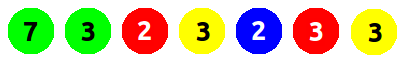
\includegraphics[scale=0.5]{fig6.png}}
\caption{7 Verde, 3 Verde, 2 Vermelho, 3 Amarelo, 2 Azul, 3 Vermelho, 3 Amarelo}
\end{figure}

A primeira coisa a se perguntar é: é possível, desde já, formar alguma estratégia, e evitar acabar jogando dentro de uma dinâmica de duplas negativa? Há sim algo a fazer, desde que se saiba de antemão como identificar quem possui um jogo mais capaz de \emph{gerenciamento}.

Dos dois jogos, o primeiro é o mais capaz disso: o jogador A possui um curinga, uma carta Comprar Duas Cartas e um Inverter, de modo que ele pode prestar atenção ao jogo e coordená-lo de acordo com sua vontade (até certo ponto). O jogador C, contudo, não tem todo esse poder bélico. Se o jogador A for capaz de comunicar que seu jogo é um jogo bom em termos de gerenciamento, então está formada uma estratégia de Divisão de Tarefas.

Caso nenhum dos dois jogos se mostrasse obviamente superior em termos de gerenciamento (seja porque ambos os jogos são ruins para tal ou bons), então deve-se esperar uma rodada, duas, ou mais, para ver quem deverá correr e quem deverá dar cobertura.

O jogador A começa o jogo. Suponha que ele saiba que ele vai ser o parceiro a gerenciar o jogo, facilitando as jogadas do jogador C. A carta na pilha de descarte é o 2 azul; você deve jogar o 5 azul, o 7 azul ou o Comprar Duas Cartas Azul. Como você deve se lembrar, jogar uma carta de compra logo no começo não é a estratégia mais recomendada, e uma vez que o jogador A já possui um outro 7, ele pode jogar o 7 Azul para auxiliar a continuidade do seu próprio jogo --- afinal, não é porque você deve priorizar a continuidade da dupla que você deve sempre esquecer da sua. Considere também que o jogo está apenas começando.

É a vez do jogador C, e a carta na pilha é um 5 azul. Não há outra opção, se ele quiser continuar jogando (e lembre-se que esse deve ser o objetivo dele: continuar jogando, inexoravelmente, até a vitória --- pelo menos enquanto a estratégia for esta). Ele joga sua única carta azul (um 2).

Como estamos considerando um exemplo de \emph{boa estratégia}, vamos considerar que o jogador C consiga emitir um sinal para o jogador A (e se fazer entender) demonstrando que esta é sua última carta azul. Lembre-se: o jogador A é responsável por tentar fazer, o quanto puder, que o jogador C continue jogando. Esta é, portanto, uma informação muito valiosa --- e seria péssimo que esse sinal fosse interceptado pelos adversários.

A carta agora é um 2 Amarelo, e é a vez do jogador A. Isso é bom; não é uma carta azul. Entretanto, ele não tem o que jogar, a não ser um Curinga. Como o Curinga pode ser muito mais útil em um estágio mais avançado do jogo, ele compra uma carta. Que mal pode haver? Será uma oportunidade de, quem sabe, ganhar mais uma carta de ataque, que pode ser mais útil.Infelizmente, é apenas um 8 vermelho.

Nossa dupla é surpreendida: o jogador C é pulado com uma carta Pular Amarela. Depois que o último adversário jogou, é a vez do jogador A novamente. Há um 9 amarelo na pilha de descarte. Você joga seu 9 vermelho, na esperança de, quem sabe, atacar algum plano do jogador B.

O jogador B joga um 9 Amarelo e o jogador C pode jogar: a estratégia continua. Ele joga um 3 Amarelo (uma vez que até possui outro). O jogador D inverte o jogo --- sorte, uma estratégia inadvertidamente prejudicial ou falta de coordenação: qualquer uma das coisas se sucede e o jogador C jova mais uma vez. Outro 3 amarelo e agora as coisas começam a se complicar; o jogador C faz um sinal para o jogador A: as cartas amarelas acabaram.

O jogador B não consegue jogar e agora é a vez do jogador A, que deve mudar a cor da carta para tentar garantir que o jogador C continue jogando. O jogador A joga o Curinga e pede pela cor verde. O Jogador D joga um 2 verde, e o jogador C pode então jogar um 3 Verde.

Podemos, antes de analisar as próximas jogadas, fazer um balanço do jogo e confirmar a importâncida coordenação da equipe. Se a divisão de tarefas não fosse empregada (e se não houvesse ocorrido uma excelente comunicação entre parceiros), o jogador A poderia fazer diversas jogadas visando a própria continudade, o que atrapalharia o jogador C --- ou ter deixado de jogar para ajudar o próprio parceiro, o que teria atrasado mais a dupla. Nesse momento, o jogador A tem 5 cartas, e o jogador C, 3. O jogador B, prestes a jogar, tem 5 cartas, e o jogador D, outras 3.

O jogador B pula o jogador A; o jogador D pula o jogador C e o jogador B usa mais uma carta Pular (foi uma sequência de cartas Pular; uma verde, uma vermelha e uma azul) para pular o jogador A e agora o turno é do jogador D novamente. Ele joga uma carta Inverter e fica com apenas uma carta na mão (não esquecendo de declarar-se ``UNO'').

O jogador A se vê numa situação complicada: ele é o responsável por gerenciar o jogo, e deve fazer algo quanto a isso. O próximo a jogar é o jogador B. Ele pode inverter o jogo, mas então o próximo a jogar seria o jogador D --- justamente aquele que possui apenas uma carta. Seria bom se o jogador A pudesse saber qual é a carta do jogador D, pois se ela não fosse verde (ou um Inverter) ele forçaria o jogador D a comprar uma carta. Entretanto, ao não prestar atenção no jogo (contando cartas) e ao não ter ocorrido um momento em que o jogador D se mostrou carente de cartas verdes (o que incorreria numa possibilidade alta de sucesso no ataque), não há como saber disso. É arriscado demais voltar o jogo para o jogador D.

Em compensação, se ele deixar o jogo correr, o jogador C não vai possuir nenhuma carta que possa prejudicar o jogador D.

Há outras duas cartas que possam ser jogadas: um 5 Azul --- inócuo nesse cenário --- e um Comprar Duas Cartas Azul. A questão é que jogar um Comprar Duas Cartas Azul faria com que o jogador \emph{B} --- e não o \emph{D} --- comprasse duas cartas, o que não seria exatamente o ideal. Além disso, a carta no topo da pilha de descarte seria azul, e o jogador C não possui mais cartas azuis.

Entretanto, isso, vai forçar o jogador C a comprar uma carta, e quem sabe essa carta não será uma carta que possa fazer com que o jogador D perca? Embora não tenha contado, com precisão, as cartas do jogo, o jogador A percebeu que \emph{nenhuma carta Curinga Comprar Quatro Cartas ou Comprar Duas Cartas, de qualquer cor, foi usada}. Dessa forma, há mais chance de que essas cartas ainda estejam no monte de compras. O Jogador A, portanto, decide por fazer com que o jogador B compre duas cartas.

É a vez do jogador C e, infelizmente, ele compra um 4 Vermelho. Com sorte, o jogador D não consegue vencer o jogo com a carta que tem à mão (note que na pilha de descarte está o Comprar Duas Cartas Azul). O jogo continua.

Para aqueles que possam pensar que de nada adianta a técnica se a dupla quase perdeu, lembre-se que o UNO também incorpora o fator da sorte e do acaso. E, ademais, estamos acompanhando apenas a trajetória de uma das duplas, não sabendo que relevância teve a estratégia da \emph{outra} dupla na configuração deste cenário.

O jogador D compra uma carta, entretanto, que ele pode jogar: um 4 Azul. Mais uma vez ele possui apenas uma carta na mão. Sabendo que ela não é azul, há agora mais chances de ela ser verde: jogar o Inverter Verde tornou-se ainda mais arriscado (sem falar que, no momento presente, impossível devido ao 4 Azul na pilha de descarte).

Declaradamente, a estratégia não mudou: o jogador A continua a tentar gerenciar o jogo. Jogar uo 5 Azul seria inútil, além de não mudar a cor da carta (atitude preferível, uma vez que o jogador C continua sem cartas azuis). O jogador A resolve, portanto, tentar a sorte mais uma vez: ele compra uma carta. É um Comprar Duas Cartas Amarelo que, infelizmente, não pode ser jogado agora.

O jogador B joga um 8 Azul. O jogador C compra um 4 Amarelo; não pode jogar. Mais uma vez, o jogador D não consegue ganhar e compra uma outra carta, que ele joga: é um Curinga. Ele pede a cor Vermelha.

O jogador A se vê em maus lençóis: as únicas cartas vermelhas que tem são inofensivas, e ele não pode jogar nada diferente frente ao Curinga na pilha de descarte. Ele compra mais uma carta: um 1 Vermelho. Não é o suficiente.

O jogador B joga um 8 Vermelho. Com a situação crítica, é mais do que sensato abandonar a divisão de tarefas e tentar gerenciar o jogo: é claro que o jogador C possui cartas vermelhas para jogar (3 delas), mas ele resolve comprar mais uma carta no que será a derradeira tentativa de impedir a vitória da outra dupla: ele compra um 3 verde, que não pode ser jogado.

O jogador D joga, enfim, seu 9 Vermelho, garantindo a vitória da dupla B e D. Como lição deste jogo-exemplo, vemos que embora a estratégia geralmente decida o jogo, a sorte também é importante. Por outro lado, não acompanhamos a dinâmica de dupla da dupla vencedora, que pode ter sido simplesmente superior. Além disso, em um jogo de parceiros existem vários outros sinais, e o fato de que alguns sinais podem ser interceptados --- ou, pior, interceptados, mas mal-interpretados --- adicionam ao jogo um fator de aleatoriedade e uma gama de possibilidades impossível de replicar em jogos-exemplo como esse.

\section{Sinais}

Já discutimos, no jogo-exemplo anterior, que tipos de sinais podem ser úteis aos parceiros durante o jogo. Vamos discutir mais em profundidade estes sinais nesta seção.

Existe uma característica fundamental de todo sinal: a profundidade de detalhes com a qual relata para o outro jogador o próprio jogo. Portanto, um sinal extremamente raso indica apenas se um jogo está ``bom'' ou ``ruim''; um sinal extremamente profundo diz ao parceiro exatamente quais são as suas cartas. Sinais rasos são difíceis de interpretar (por parte dos adversários ou, se não houver combinação prévia, por parte do próprio parceiro), ao passo que quanto mais profundo um sinal, mais difícil será de fazê-lo de forma discreta, ou de criptografá-lo a ponto de criar dificuldades para que os adversários o entendam. Alguns sinais, contudo, não precisam ser explícitos: podem ser mascarados como cacoetes, como coçar a bochecha ou a cabeça, e são mais eficientemente mascarados se você não olha para o seu parceiro enquanto os executa (embora isso exija um nível de cumplicidade enorme: você não terá certeza se o parceiro entendeu o sinal ou mesmo se o viu).

Seja como for que o sinal seja feito, é útil saber que tipo de informação, não muito rasa, mas também não muito profunda a ponto de necessitar de sinais complexos, pode ser útil para o parceiro em um jogo de duplas:

\begin{description}
\item[Número de Cartas de Ataque]{Quantas cartas de ataque (Inverter, Pular, Comprar Duas, Comprar Quatro) você possui (ou não possui, caso não possua nenhuma). Pode ser útil para definir quem gerencia o jogo.}
\item[Número de Cartas Pular]{Quantas cartas Pular você possui. Útil para uma eventual formação de um Isolamento (ver adiante).}
\item[Comprei uma Carta de Ataque]{Informe ao parceiro que você comprou algo interessante. Se possível, diga que tipo de carta, ou apenas diferencie entre Pular/Inverter e alguma carta que force o adversário a comprar cartas --- ou diga se é um Curinga ou não.}
\item[Sem esta Cor]{Indicar, de alguma forma, quando você não tem mais uma cor em sua mão. Algo como uma coçada na nuca quando a cor estiver na pilha de descarte já funciona.}
\item[Que Cor?]{Quando o parceiro puder escolher uma cor (por meio de um Curinga), e você tiver alguma preferência, pode indicar que cor prefere.}
\item[Mude a Cor]{Se por algum motivo (não necessariamente por ser a cor que você não tem) seja uma boa ideia mudar a cor na pilha de descarte, é uma boa ideia informar ao parceiro.}
\end{description}

\section{Estratégias Específicas de Jogo de Parceiros}

A maioria das estratégias específicas, empregadas em um jogo individual, pode ser traduzida em estratagemas análogos, porém utilizando todas as possibilidades do jogo em duplas.

\subsection{O Curinga Facilitado}

\label{curingafacil}

Quando o Curinga Surpresa (ver acima, na página \pageref{curingasurpresa}) é empregado, um dos jogadores precisa contar com certa sorte: precisa jogar de modo a fazer com que sua continuidade dê certo, sem poder controlar o jogo, guardando o Curinga para que ele seja a última carta.

Num jogo de duplas, contudo, quando uma equipe possui alguém que claramente é o gerenciador do jogo e o outro que é aquele que deve se livrar das cartas (e este último possui um Curinga), essa estratégia passa a precisar menos de sorte, e mais de companheirismo e perspicácia. No Curinga Facilitado, o jogador gerenciador controla o jogo de modo a permitir que o outro jogador da mesma equipe conserve seu curinga e jogue-o na última rodada. 

\subsection{``Olha o Avião'' Curto}

\label{aviaocurto}

\begin{wrapfigure}{o}{0.25\textwidth}
  \begin{center}
    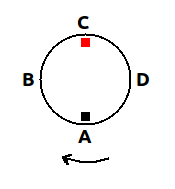
\includegraphics[scale=0.5]{fig7.png}
  \end{center}
  \caption{O jogador A joga um curinga. O jogador C, parceiro, precisa de ou quer uma carta vermelha. Ao pedir uma carta de outra cor, confunde o jogador B.}
\end{wrapfigure}

O Olha o Avião longo (ver página \pageref{aviaolongo}), empregado no jogo individual, pode ser empregado também em um jogo de duplas em uma situação muito particular.

Imaginemos novamente um jogo-exemplo, com os jogadores A, B, C e D (duplas A e C, B e D). O jogador A escolhe a cor para a próxima jogada. O jogador B é o próximo a jogar. O jogador C, da equipe do jogador A, pode ganhar o jogo (ou tem duas, três cartas na mão).

Se for provável que o jogador B seja o jogador gerenciador na dupla adversária --- ou que, naquele momento, esteja, de alguma forma, claro que ele tentará inverter a cor para que o jogador C não consiga jogar, uma boa estratégia é apostar na requisição de uma cor estranha, que mesmo o jogador C não tenha (ou que não seja a melhor escolha possível). O jogador B inverte as cores, escolhendo uma que talvez seja justamente a melhor cor para a situação.

\subsection{Zero em Duplas}

O mesmo conselho pode ser dado quanto ao zero, tanto em jogos individuais como em duplas: conserve se o momento não for favorável, descarte o mais rápido possível em nome da continuidade. Entretanto, em um jogo de parcerias, se um dos jogadores estiver em posição de gerenciar o jogo, e o zero estiver nas mãos do outro parceiro, então a situação não é tão ameaçadora, e o zero pode ser conservado por mais tempo. 

\subsection{Trébuchet Duplo}

\label{trebuchetduplo}

Assim como os tipos de Trébuchet vistos anteriormente (páginas \pageref{trebuchetlongo} e \pageref{trebuchetcurto}), essa estratégia, que na mairoia das vezes surge de forma acidental, também pode ocorrer em um jogo de duplas. É possível que ninguém possua uma carta adequada para jogar, e então todos comprem durante duas ou três rodadas, o que pode ser muito vantajoso para uma dupla, embora não para outra (embora nem sempre este seja o caso).

No Trébuchet Duplo, contudo, vale a pena destacar algumas diferenças: Em primeiro lugar, é preciso que a dupla esteja unida nessa estratégia; se um dos jogadores a vê e a utiliza, é preciso que seu parceiro também colabore, se não de nada adiantará o esforço individual do primeiro.

Além disso, o fato de que as jogadas dos dois jogadores de uma dupla forcem os outros jogadores a comprar não constitui um Trébuchet; um Trébuchet é quando \emph{todos} compram. Estratégias deste outro tipo serão abordados de agora em adiante.

\subsection{Abastecimento}

A estratégia do abastecimento pode ser empregada mediante uma série de fatores e é difícil de funcionar bem por um longo tempo. Em geral, é antes um princípio de ação do que uma estratégia, uma vez que se pode agir de modo a tentar ``abastecer'' um adversário, mas dificilmente se poderá manter essa dinâmica de jogo sem prejuízo à estratégia maior da dupla, que é, evidentemente, a vitória.

O abastecimento consiste em jogadas feitas com o objetivo de forçar um adversário (ou até mesmo os dois, embora isto seja muito mais complexo) a comprar cartas. O alvo preferencial será escolhido de acordo com seu número de cartas (quanto menor, mais importante é que seja abastecido) e também de acordo com a característica das suas cartas no momento.

O abastecimento envolve, portanto, a coordenação da dupla em prol de jogadas que forcem um jogador a comprar cartas. Vamos voltar ao modelo de jogo exemplo com o qual temos trabalhado: duplas entre os jogadores A e C, e entre os jogadores B e D.

O jogador A joga uma carta esperando, de alguma forma, facilitar uma jogada do jogador C em que ele force o jogador D a comprar --- ou seja, o jogador A tenta proporcionar ao jogador C a change de jogar uma carta que force o jogador D a comprar duas ou quatro cartas, ou ainda uma carta de uma cor que o jogador D seguramente não tem (aumentando as chances de que o jogador D tenha que comprar uma carta).

O abastecimento, portanto, depende das condições do adversário alvo: se ele está vulnerável ao não ter diversos tipos de cartas para jogar. Também depende de sua possibilidade de ganhar o jogo; gastar tempo abastecendo um jogador cheio de cartas é prejudicial, uma vez que isso pode eventualmente ajudá-lo a assumir uma posição de gerenciamento do jogo que acabará por prejudicar a dupla que o abasteceu.

\subsection{Isolamento}

O isolamento, ao contrário do abastecimento, não consiste em fazer com que um dos jogadores da dupla adversária compre mais cartas, mas, ao invés disso, tenta fazer com que eles não joguem. O isolamento, por tanto, é uma técnica que se utiliza de cartas Pular.

O Isolamento simples é o mais fácil de ocorrer: em uma dupla, um dos jogadores possui duas ou mais cartas Pular. Vamos supor que o jogador A possua três cartas Pular; ele pula o jogador B. O jogador C joga de modo a proporcionar ao jogador A a chance de jogar outra carta Pular, que de fato é jogada; o mesmo acontece na próxima rodada e o jogador B deixa de jogar por três rodadas seguidas. Um jogador foi ``isolado'' do jogo.

Isso é extremamente benéfico pois faz com que um jogador continue com muitas cartas na mão (não apenas para afastar dele a chance de vitória mas também para, em um caso de vitória da dupla de ataque, muitos pontos serem obtidos), faz com que o jogo esteja ainda mais sob controle por parte da dupla de ataque, e deixa sem reforços o outro jogador da dupla. Por outro lado, o que é um aspecto que pode ser tanto positivo quanto negativo, o jogador isolado pode se deixar levar pelas emoções, pretendendo, portanto, atacar de forma mais violenta (como visto acima na seção ``O Estímulo Passional'').

Se um jogador possui três cartas Pular e as joga em diferentes momentos do jogo, isso não é considerado um Isolamento. O isolamento é o uso repetitivo, seguido, de cartas Pular para, de forma prolongada, impedir um jogador específico de jogar. Ele, portanto, se diferencia do uso avulso destas cartas de ação por essa característica tática não existente no emprego aleatório (ou com base em outro princípio) das cartas em questão.

\subsection{Isolamento Sistemático}

O isolamento sistemático é uma variante mais rara do isolamento, em que ambos os jogadores das duplas possuem uma certa quantidade de cartas Pular, e as usam de forma simultânea para descartar várias cartas e, ao mesmo tempo, impedir que a outra dupla jogue.

Ao final de um isolamento sistemático, percebe-se que é como se o jogo tivesse sido paralisado e retornado ao normal, porém com uma das duplas com várias cartas a menos. É, portanto, um ataque muito vantajoso, porém difícil de ser empregado por causa das condições raras em que ele pode ser executado.

\subsection{Isolamento Fatal}

O isolamento fatal é uma espécie de isolamento sistemático, em que a mesma lógica do ``Curinga Surpresa'' é aplicada: a dupla deixa, como as últimas cartas em suas mãos, cartas Pular que são usadas para realizar um Isolamento Sistemático, de forma que assim, com três cartas na mão de um jogador e até mesmo quatro na mão de outro, uma dupla pode vencer de modo surpreendente com este ataque fulminante, ao qual é absolutamente impossível reagir uma vez que tenha sido iniciado. É ainda mais difícil de realizar do que um Isolamento Sistemático, uma vez que precise que ambos os jogadores tenham no mínimo duas cartas Pular, e tenham tido condições de deixá-las por último.

Tanto o abastecimento quanto o isolamento não foram discutidos no jogo de cunho individual por não fazerem sentido em um jogo deste tipo: em um jogo com 5 pessoas, uma pode até mesmo ``isolar'' um jogador (o próximo na sequência de jogadas, caso ela não se altere) ao impedi-lo repetidamente de jogar, mas isso não possui um efeito estratégico muito interessante, pois ele ainda precisa lidar com outros 3 jogadores, cujas estratégias de nada dependem desse único adversário afetado. No jogo em parcerias, contudo, atacar um dos jogadores constitui um ataque direto à estrutura de uma espécie de adversário único que é a outra dupla.

\section{Jogo de Várias Parcerias}

É possível jogar UNO com mais de duas duplas de parceiros; só o que é requerido é que os parceiros sentem-se de frente um para o outro na disposição da mesa. Esse é um tipo de jogo extremamente complexo em que a mesma estratégia geral (de continuidade e gerenciamento) são válidos, mas com menos possibilidades de controle  e mais variáveis para prestar atenção.

Das estratégias específicas para o jogo de duplas algumas são válidas, mas outras não o são --- e outras o são parcialmente. 

O Curinga Facilitado (ver acima, na página \pageref{curingafacil}) ainda é possível, mas com muito mais dificuldade, pois dois jogadores (ou mais) se interpõem aos jogadores da mesma dupla. O Trébuchet (ver acima, nas páginas \pageref{trebuchetlongo}, \pageref{trebuchetcurto} e \pageref{trebuchetduplo}) também pode vir a acontecer, mas é um acontecimento mais raro.

A tática do Olha o Avião (ver na página \pageref{aviaolongo} e especialmente na página \pageref{aviaocurto}) continua sendo possível. O abastecimento também prossegue sendo possível, porém com um nível maior de dificuldade, e todos os tipos de isolamento são muito mais difíceis de fazer: só é possível isolar todas as duplas que se interpõem entre dois parceiros se a regra do Descarte Rápido ou das Duplicatas for usada (ver as regras abaixo nas páginas \pageref{descarterapido} e \pageref{duplicatas}).